\section{Interactive Adverts}
In this section we will show screen grabs of all stages of the interaction process within each advert and provide a sampling of feedback comments from our user study.

\subsection{Fosters}
	\begin{description}
		\item[On Load]{A Facebook ``Like'' button is present in the lower right hand part of the screen. See \ref{fig:fosters1}.}
		\item[On Clicking the ``Like Button'']{``Like'' button visually changes to indicate that the product has been liked. See \ref{fig:fosters2}.}
	\end{description}
	
	\begin{figure}[th]
		\centering
		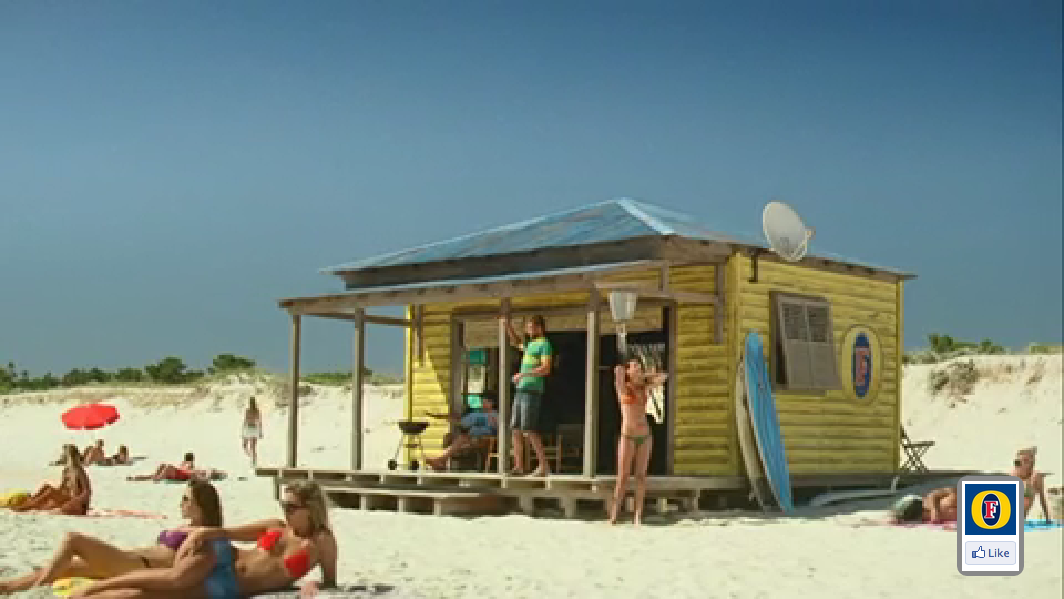
\includegraphics[width=\textwidth,height=0.5\textheight,keepaspectratio]{images/adverts/fosters-1.png}
		\caption{Fosters advert, before liking.}
		\label{fig:fosters1}
	\end{figure}
	
	\begin{figure}[th]
		\centering
		
\includegraphics[width=\textwidth,height=0.5\textheight,keepaspectratio]{images/adverts/fosters-2.png}
		\caption{Fosters advert, after liking.}
		\label{fig:fosters2}
	\end{figure}
	
\subsection{Dominoes}
	\begin{description}
		\item[On Load]{Modified Dominoes logo shown in top left including the phrase ``Fancy Domino's Pizza? Tap here!'' See \ref{fig:Dominos1}.}
		\item[On Tapping the logo]{Logo is replaced by a Pizza cut into 4 sections, each annotated with the phrase ``Tap to Order''. Each section displays a different type of dominoes Pizza. See \ref{fig:Dominos2}.}
		\item[On Tapping a Pizza Segment]{The graphic is removed and text is displayed reading: ``Your Pizza is on its way!'' See \ref{fig:Dominos3}.}
		\item[On Timeout]{Text fades away leaving the advert unobstructed.}
	\end{description}
	
	\begin{figure}[th]
		\centering
		
\includegraphics[width=\textwidth,height=0.5\textheight,keepaspectratio]{images/adverts/dominos-1.png}
		\caption{Domino's advert, before interaction.}
		\label{fig:Dominos1}
	\end{figure}
	
	\begin{figure}[th]
		\centering
		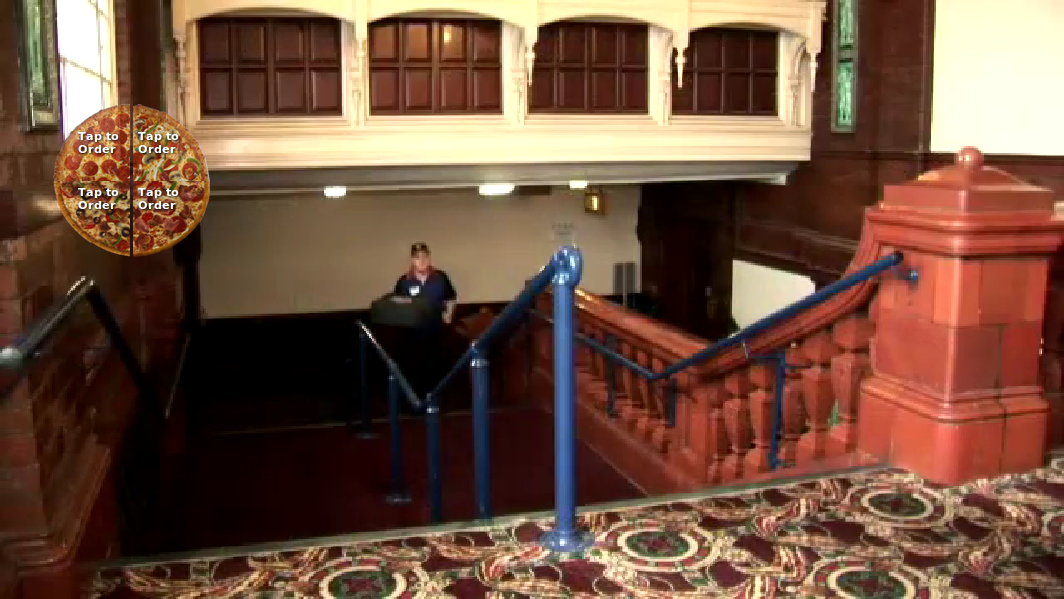
\includegraphics[width=\textwidth,height=0.5\textheight,keepaspectratio]{images/adverts/dominos-2.png}
		\caption{Domino's advert, after the logo is tapped.}
		\label{fig:Dominos2}
	\end{figure}
	
	\begin{figure}[th]
		\centering
		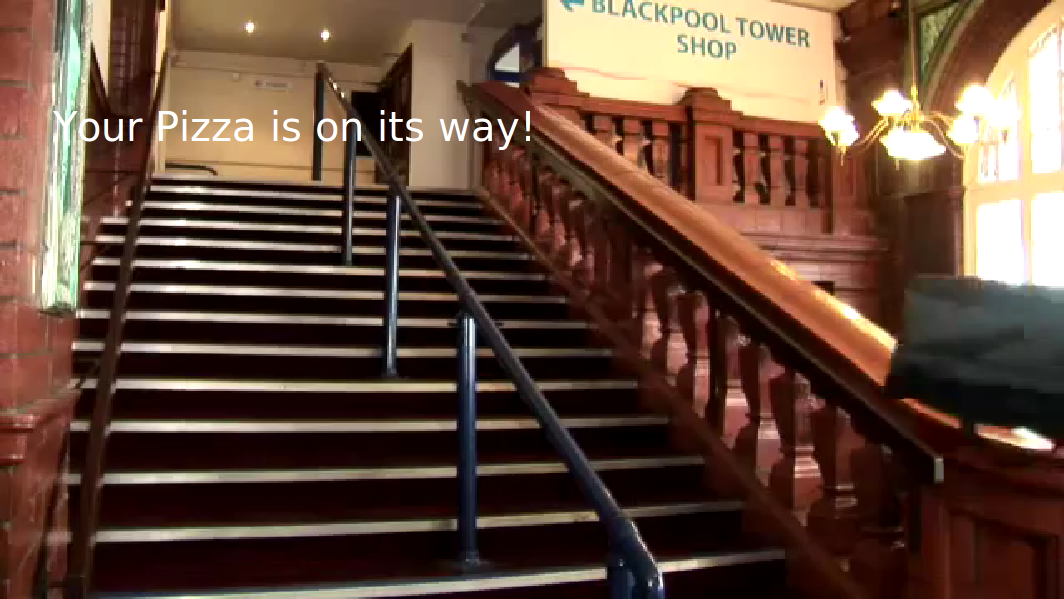
\includegraphics[width=\textwidth,height=0.5\textheight,keepaspectratio]{images/adverts/dominos-3.png}
		\caption{Domino's advert, after selecting a pizza segment.}
		\label{fig:Dominos3}
	\end{figure}
	
\subsection{Unified Insurance Cover}
	\begin{description}
		\item[On Load]{Grey, semi-transparent bar displayed along the bottom of the screen with the text ``I have...'' positioned at the left. Additionally another similar box appears in the top right with the text ``Your Quote: £0''. See \ref{fig:Paddy1}.}
		\item[On Timeout Event]{A tickbox appears first growing then shrinking into place to the right of the current content in the lower bar marked ``A laptop?'' See \ref{fig:Paddy2}.}
		\item[On Timeout Event]{A tickbox appears first growing then shrinking into place to the right of the current content in the lower bar marked ``A hifi?'' See \ref{fig:Paddy3}.}
		\item[On Timeout Event]{A tickbox appears first growing then shrinking into place to the right of the current content in the lower bar marked ``A bike?'' See \ref{fig:Paddy4}.}
		\item[On Timeout Event]{A tickbox appears first growing then shrinking into place to the right of the current content in the lower bar marked ``A console?'' See \ref{fig:Paddy5}.}
		\item[On ticking or unticking a tickbox]{The quote in the top right changes to reflect an estimated quote for someone with the items currently ticked. See \ref{fig:Paddy6} and \ref{fig:Paddy7}.}
	\end{description}
	
	\begin{figure}[th]
		\centering
		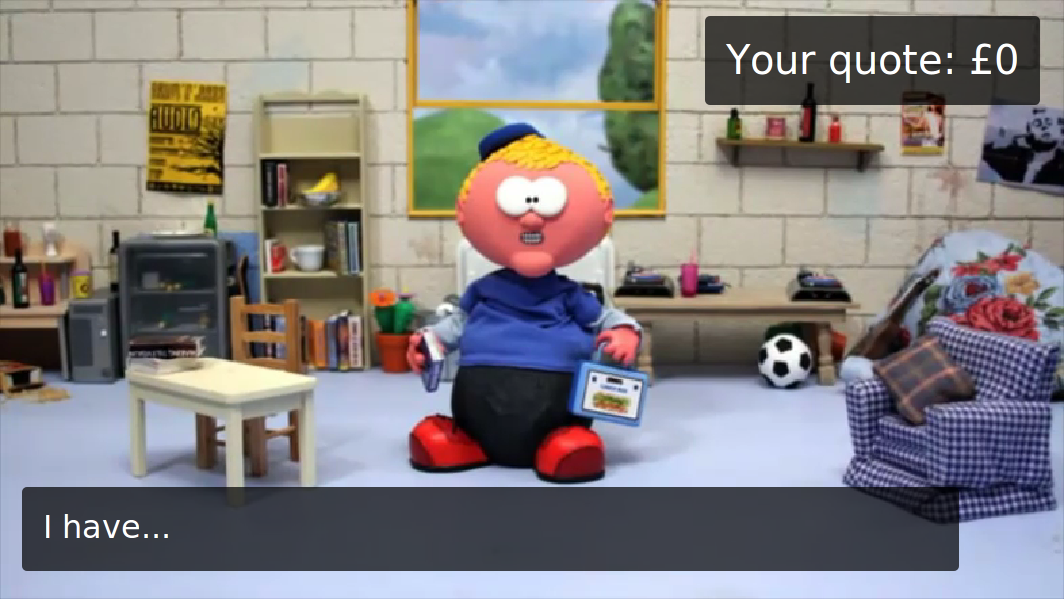
\includegraphics[width=\textwidth,height=0.5\textheight,keepaspectratio]{images/adverts/unified_insurance_cover-1.png}
		\caption{Unified Insurance Cover advert, initial.}
		\label{fig:Paddy1}
	\end{figure}
	
	\begin{figure}[th]
		\centering
		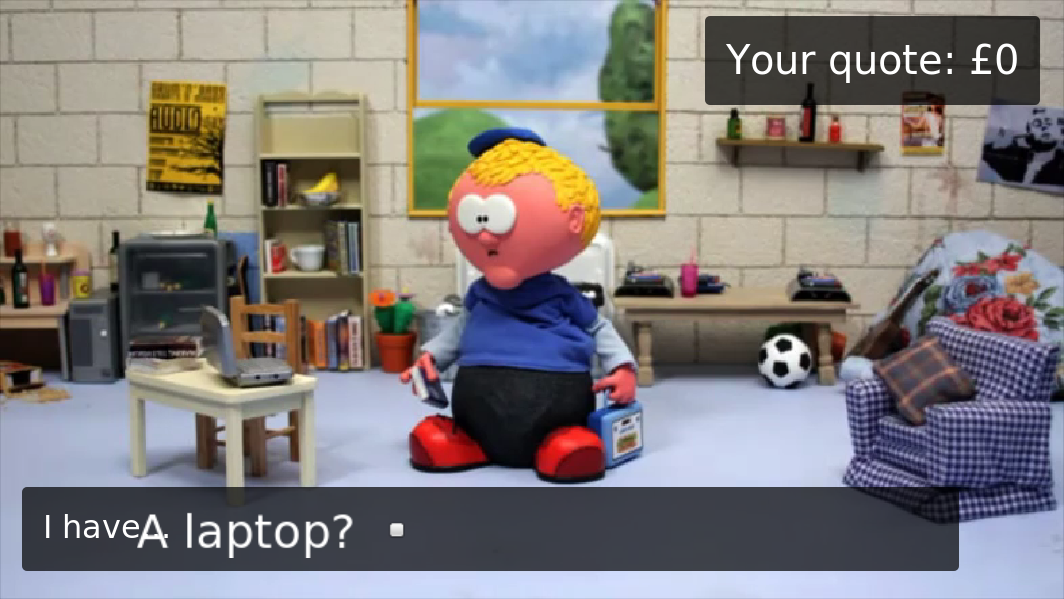
\includegraphics[width=\textwidth,height=0.5\textheight,keepaspectratio]{images/adverts/unified_insurance_cover-2.png}
		\caption{Unified Insurance Cover advert, first item added.}
		\label{fig:Paddy2}
	\end{figure}
	
	\begin{figure}[th]
		\centering
		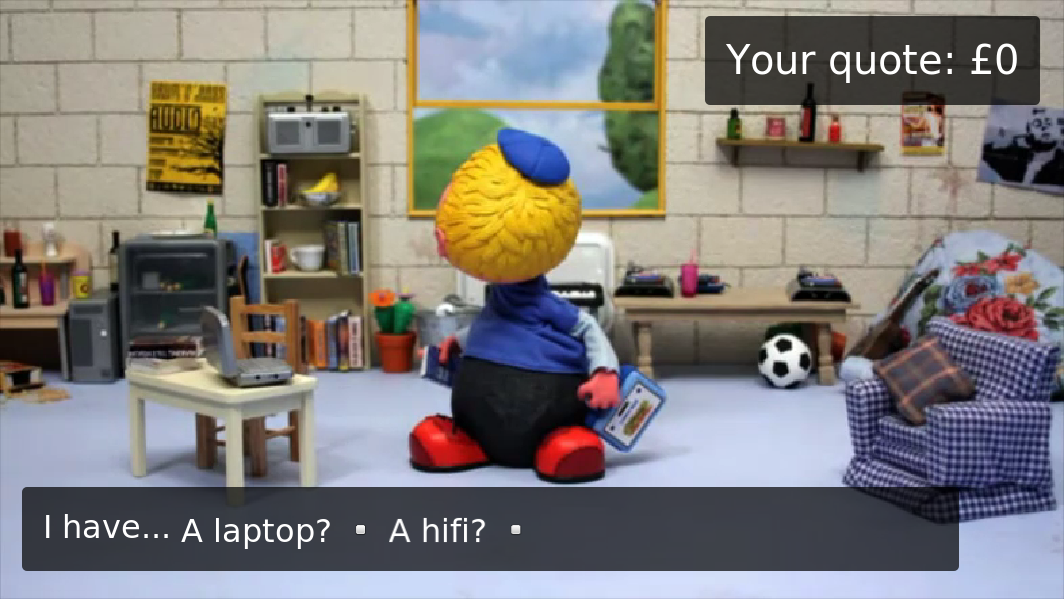
\includegraphics[width=\textwidth,height=0.5\textheight,keepaspectratio]{images/adverts/unified_insurance_cover-3.png}
		\caption{Unified Insurance Cover advert, second item added.}
		\label{fig:Paddy3}
	\end{figure}
	
	\begin{figure}[th]
		\centering
		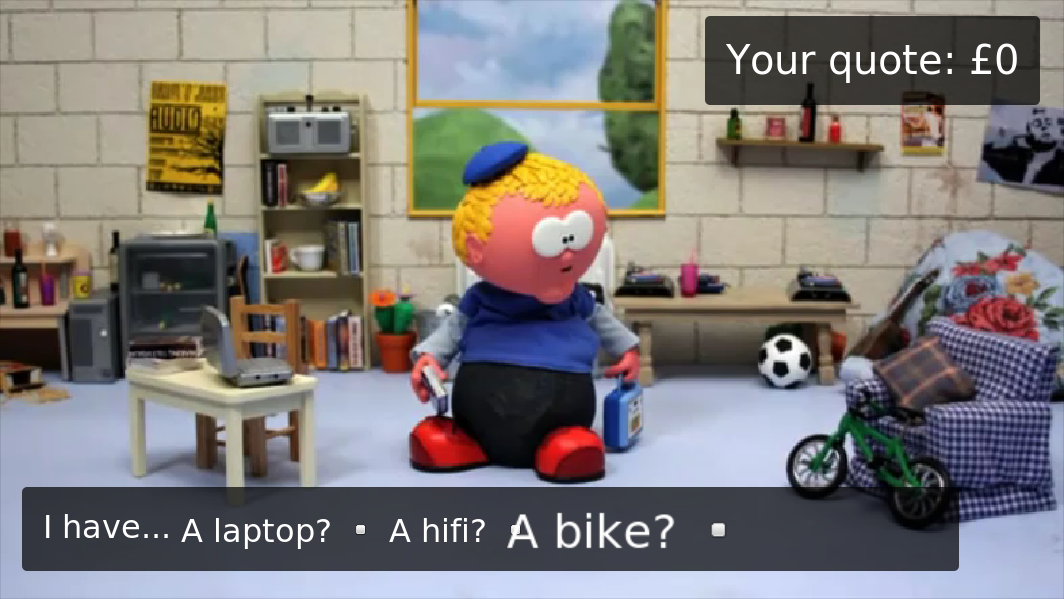
\includegraphics[width=\textwidth,height=0.5\textheight,keepaspectratio]{images/adverts/unified_insurance_cover-4.png}
		\caption{Unified Insurance Cover advert, third item added.}
		\label{fig:Paddy4}
	\end{figure}
	
	\begin{figure}[th]
		\centering
		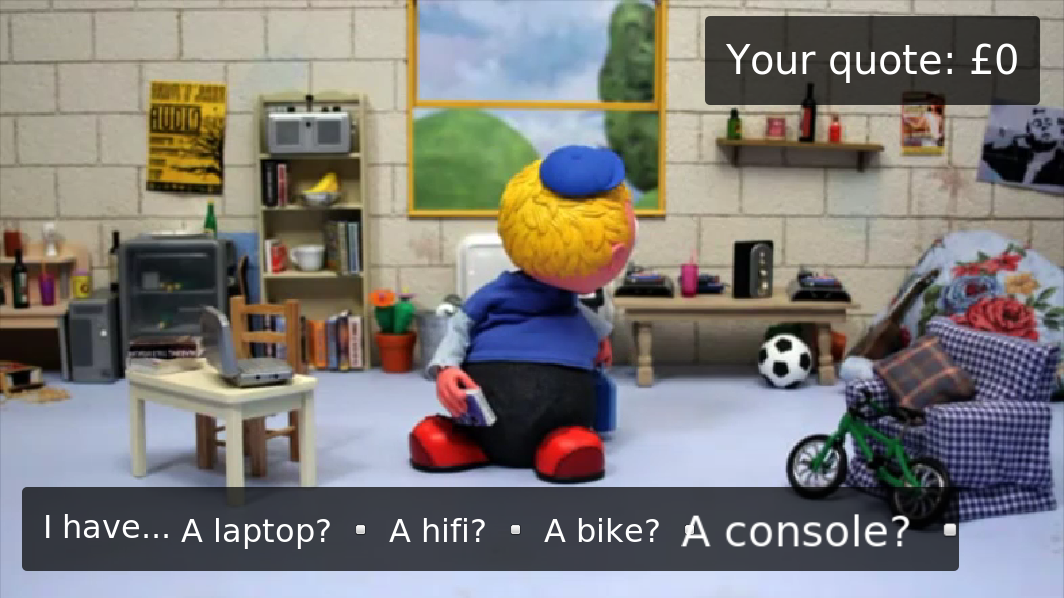
\includegraphics[width=\textwidth,height=0.5\textheight,keepaspectratio]{images/adverts/unified_insurance_cover-5.png}
		\caption{Unified Insurance Cover advert, fourth item added.}
		\label{fig:Paddy5}
	\end{figure}
	
	\begin{figure}[th]
		\centering
		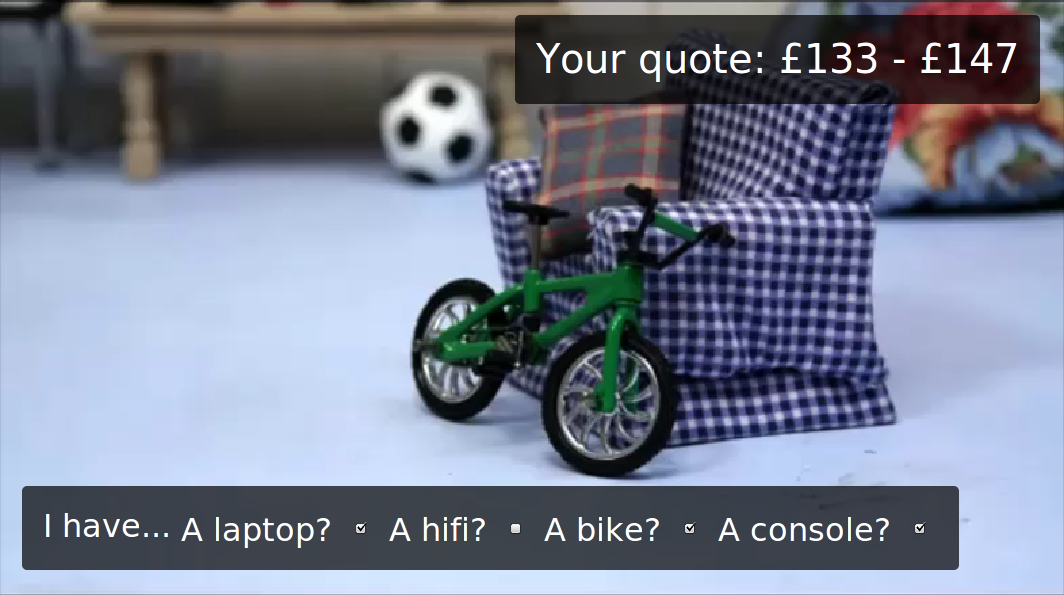
\includegraphics[width=\textwidth,height=0.5\textheight,keepaspectratio]{images/adverts/unified_insurance_cover-6.png}
		\caption{Unified Insurance Cover advert, several items ticked.}
		\label{fig:Paddy6}
	\end{figure}
	
	\begin{figure}[th]
		\centering
		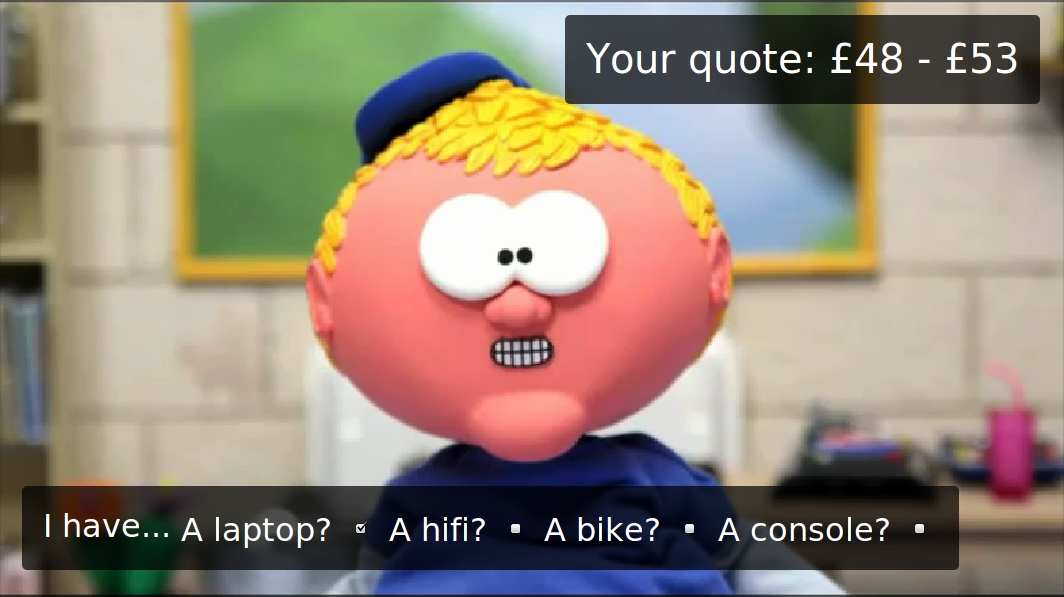
\includegraphics[width=\textwidth,height=0.5\textheight,keepaspectratio]{images/adverts/unified_insurance_cover-7.png}
		\caption{Unified Insurance Cover advert, single item ticked.}
		\label{fig:Paddy7}
	\end{figure}	
	
\subsection{thetrainline.com}
	\begin{description}
		\item[On Load]{Translucent grey box displayed on the right of the screen with the text ``Are train tickets too expensive?'' and two buttons; one green, marked ``YES'' and one red marked ``NO''. See \ref{fig:trainline1}}
		\item[On clicking either button]{The buttons are removed and replaced by a bar chart showing live results of the poll. See \ref{fig:trainline2}}
	\end{description}
	
	\begin{figure}[th]
		\centering
		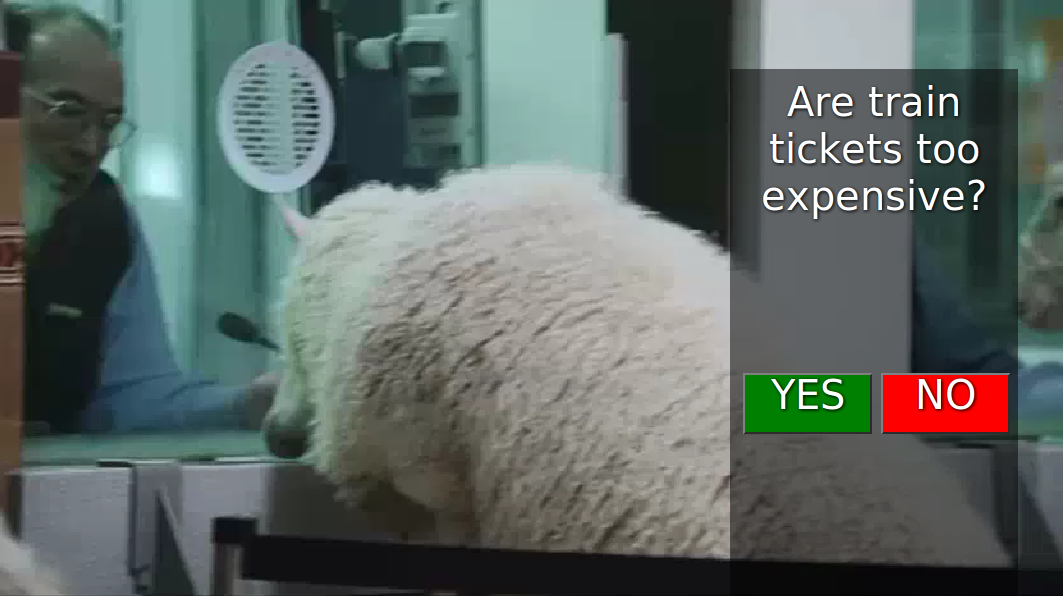
\includegraphics[width=\textwidth,height=0.5\textheight,keepaspectratio]{images/adverts/trainline-1.png}
		\caption{thetrainline.com advert, before interaction.}
		\label{fig:trainline1}
	\end{figure}
	
	\begin{figure}[th]
		\centering
		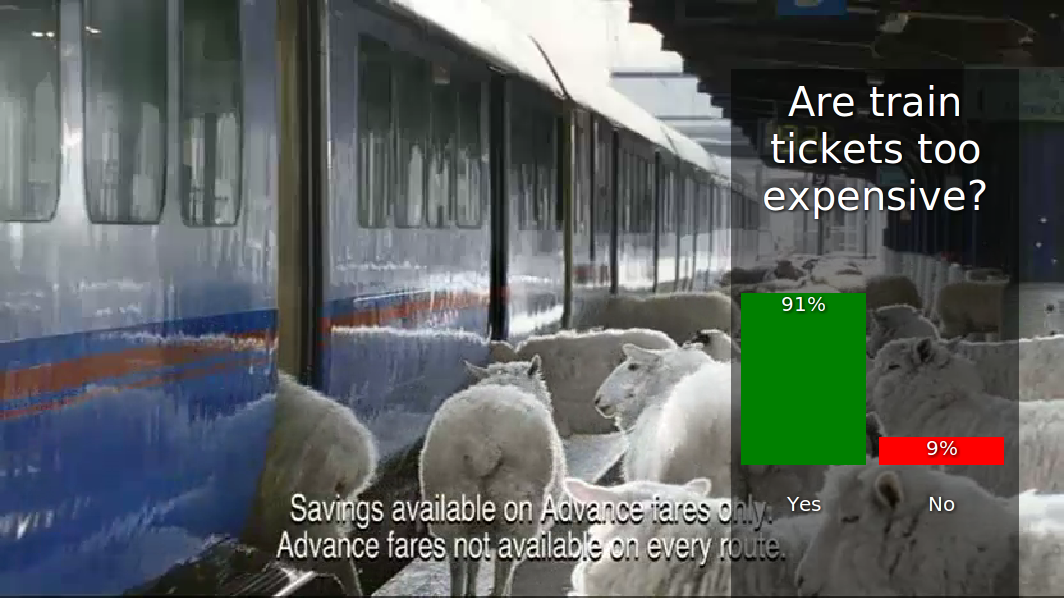
\includegraphics[width=\textwidth,height=0.5\textheight,keepaspectratio]{images/adverts/trainline-2.png}
		\caption{thetrainline.com advert, after option is selected.}
		\label{fig:trainline2}
	\end{figure}
	
\subsection{Pot Noodle}
	\begin{description}
		\item[On Load]{Grey, semi-transparent bar displayed along the bottom of the screen with the text ``BEST Pot Noodle?''. Images of 5 flavours of Pot Noodle are displayed next to this as well as a 6th image in the shape of a Pot Noodle with a ``?'' in the centre. A countdown also begins starting at ``15s'' positioned below the text. See \ref{fig:potNoodle1}.}
		\item[Every second for 15 seconds]{Countdown text updates to show 1 less second remaining.}
		\item[If user clicks a Pot Noodle image before the countdown ends]{The Pot Noodle they selected grows to emphasise that it has been selected. See \ref{fig:potNoodle2}.}		
		\item[If user clicks the same Pot Noodle image before the countdown ends that they previously selected]{The Pot Noodle they tapped shrinks to its initial size to emphasise that it has been deselected.}
		\item[If user clicks a different Pot Noodle image before the countdown ends than one that they previously selected]{The Pot Noodle they selected before shrinks to its initial size to emphasise that it has been deselected. The new Pot Noodle they selected grows to emphasise that it has been selected. See \ref{fig:potNoodle3}.}
		\item[If the countdown ends while no Pot Noodle has been chosen]{The grey bar fades out leaving the remainder of the advert unobstructed.}
		\item[If the countdown ends while a pot noodle is selected]{The gray bar fades out and the user is briefly shown some text ``Thanks for voting''. See \ref{fig:potNoodle4}.}
		\item[On Timeout]{Text fades away leaving the advert unobstructed.}
	\end{description}
	
	\begin{figure}[th]
		\centering
		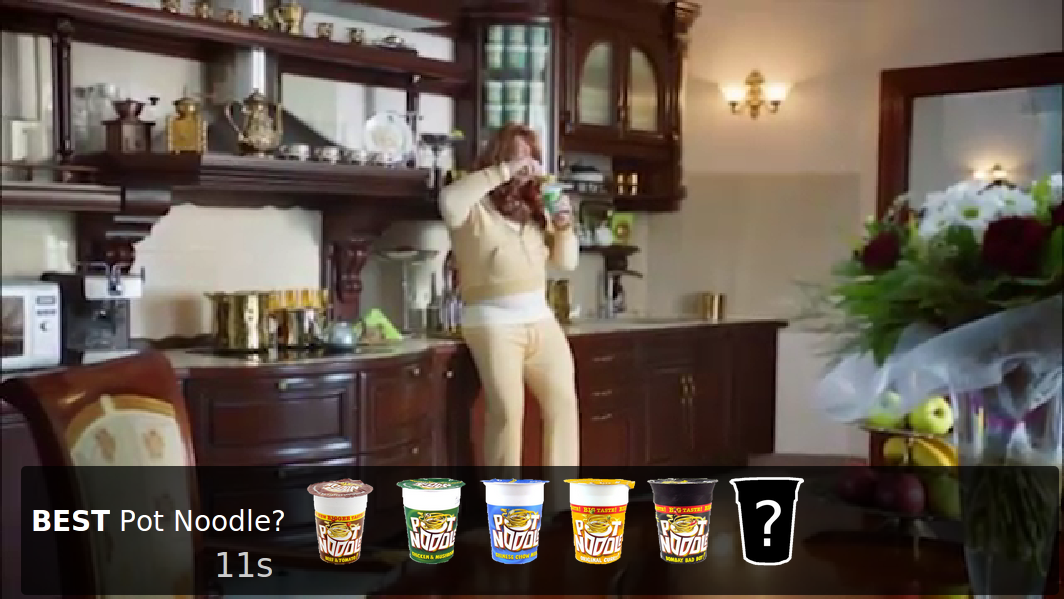
\includegraphics[width=\textwidth,height=0.5\textheight,keepaspectratio]{images/adverts/pot_noodle-1.png}
		\caption{Pot Noodle advert, before interaction.}
		\label{fig:potNoodle1}
	\end{figure}
	
	\begin{figure}[th]
		\centering
		
\includegraphics[width=\textwidth,height=0.5\textheight,keepaspectratio]{images/adverts/pot_noodle-2.png}
		\caption{Pot Noodle advert, other Pot Noodle selected.}
		\label{fig:potNoodle2}
	\end{figure}
	
	\begin{figure}[th]
		\centering
		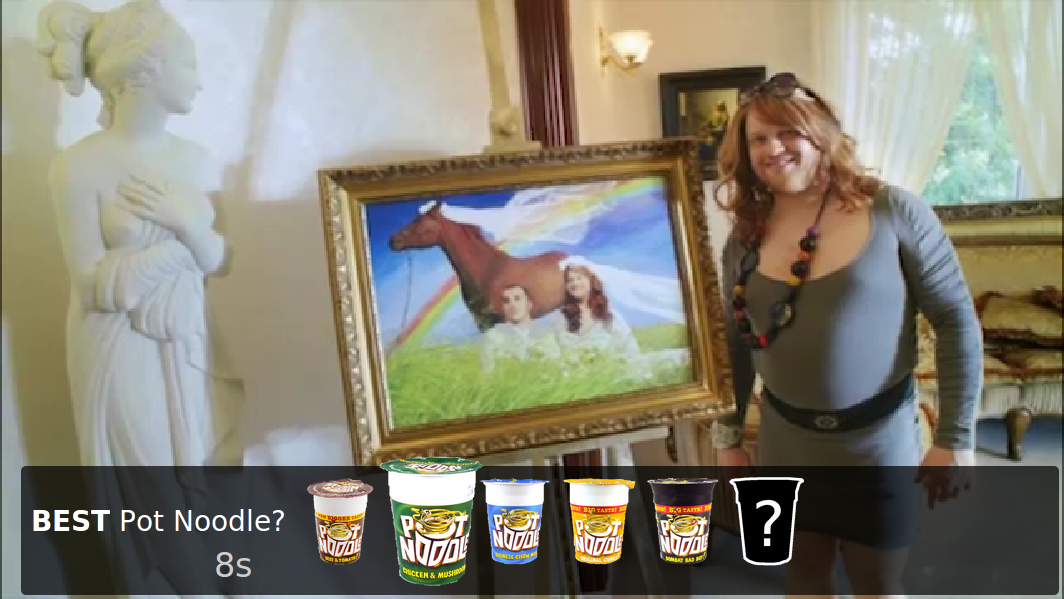
\includegraphics[width=\textwidth,height=0.5\textheight,keepaspectratio]{images/adverts/pot_noodle-3.png}
		\caption{Pot Noodle advert, Chicken and Mushroom Pot Noodle selected.}
		\label{fig:potNoodle3}
	\end{figure}
	
	\begin{figure}[th]
		\centering
		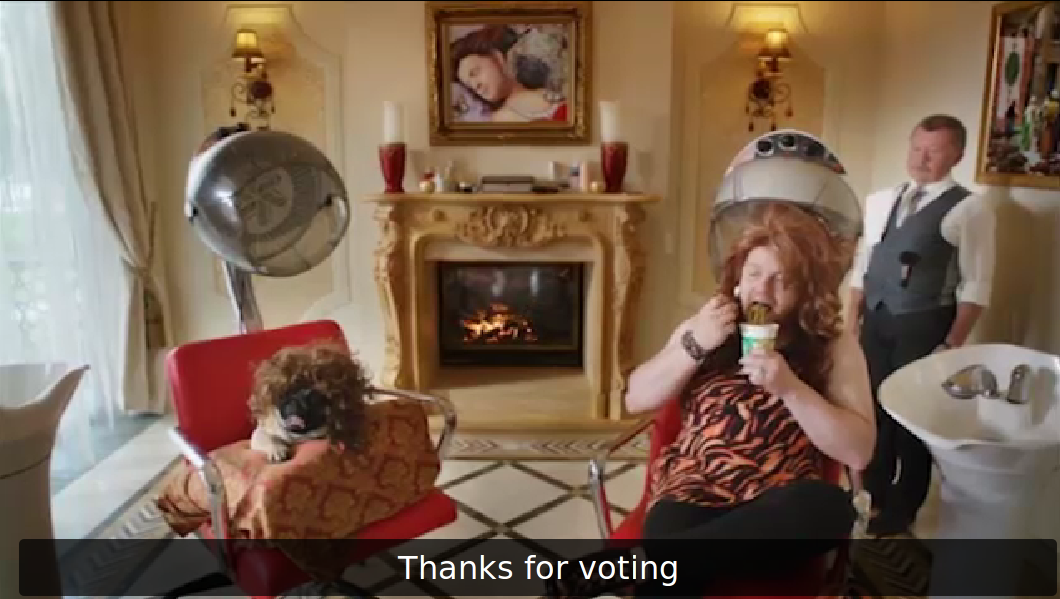
\includegraphics[width=\textwidth,height=0.5\textheight,keepaspectratio]{images/adverts/pot_noodle-4.png}
		\caption{Pot Noodle advert, after countdown ends.}
		\label{fig:potNoodle4}
	\end{figure}
	
\subsection{Smirnoff}
	\begin{description}
		\item[On Load]{A Facebook ``Like'' button is present in the lower right hand part of the screen. See \ref{fig:smirnoff1}.}
		\item[On Clicking the ``Like Button'']{``Like'' button visually changes to indicate that the product has been liked. See \ref{fig:smirnoff2}.}
	\end{description}
	
	\begin{figure}[th]
		\centering
		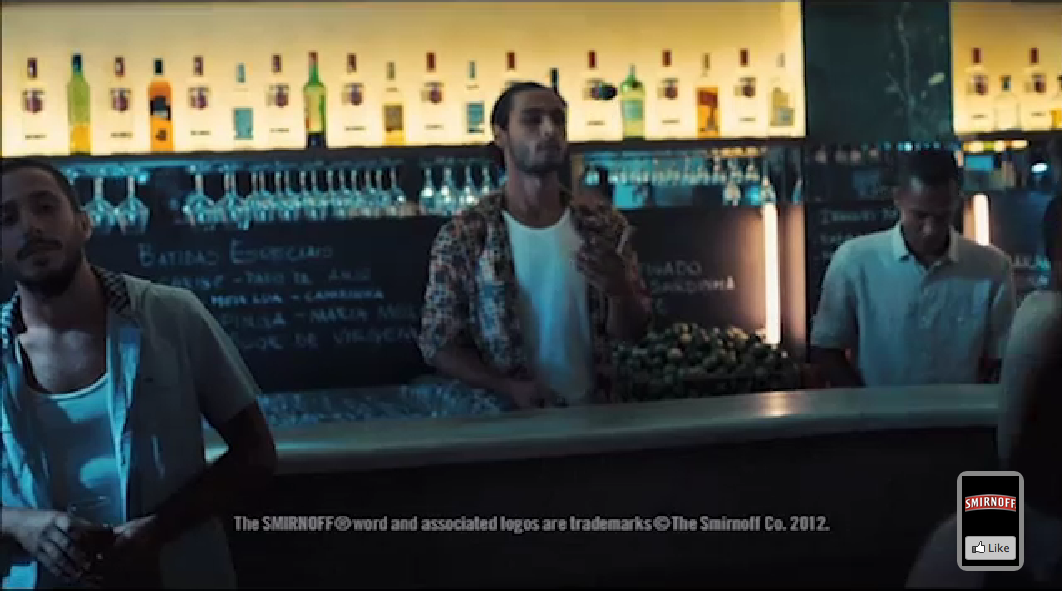
\includegraphics[width=\textwidth,height=0.5\textheight,keepaspectratio]{images/adverts/smirnoff-1.png}
		\caption{Smirnoff advert, before liking.}
		\label{fig:smirnoff1}
	\end{figure}
	
	\begin{figure}[th]
		\centering
		
\includegraphics[width=\textwidth,height=0.5\textheight,keepaspectratio]{images/adverts/smirnoff-2.png}
		\caption{Smirnoff advert, after liking.}
		\label{fig:smirnoff2}
	\end{figure}
	
\subsection{The Perks of Being a Wallflower}
	\begin{description}
		\item[On Load]{Grey, semi-transparent box displayed in the bottom left of the screen with the text ``Find nearby showings:''. Below this is a box with helper text ``postcode'' and to the right of this is a button marked ``Go''. See \ref{fig:wallflower1}.}
		\item[On clicking the ``Go'' button with a valid postcode in the postcode box]{A map is displayed, centred on the screen with markers indicating nearby cinemas showing the film. The map window comes with its own set of standard controls which may also be used. See \ref{fig:wallflower2} and \ref{fig:wallflower3}.}
		\item[On clicking the markers on the map]{A bubble appears over the marker stating the name of the cinema. See \ref{fig:wallflower4}.}
		\item[On clicking the ``X'' button]{The map view is closed, allowing the advert to be fully seen once more.}
	\end{description}
	
	\begin{figure}[th]
		\centering
		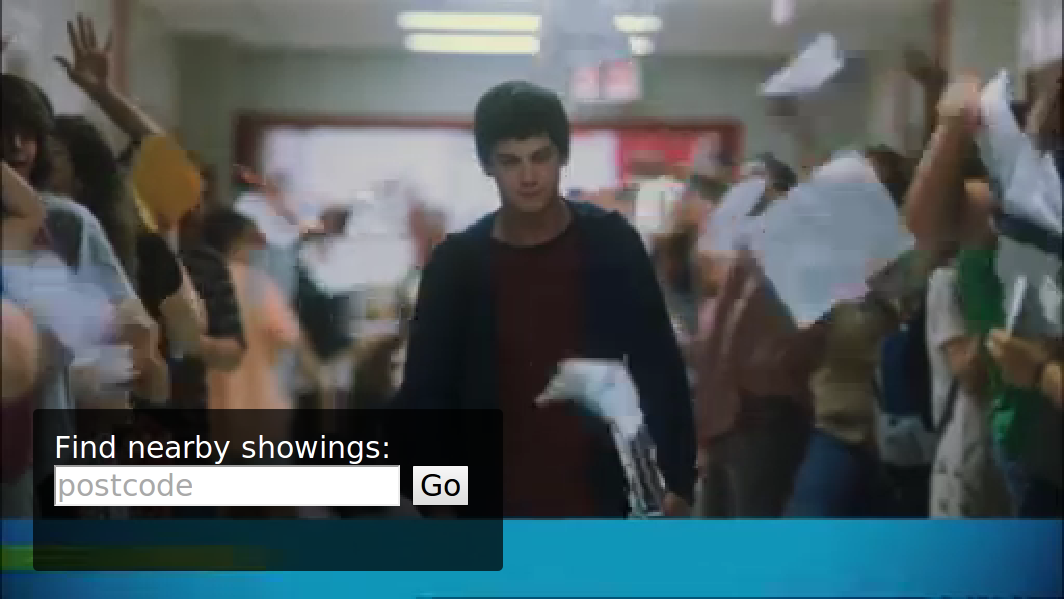
\includegraphics[width=\textwidth,height=0.5\textheight,keepaspectratio]{images/adverts/wallflower-1.png}
		\caption{The Perks of Being a Wallflower film advert, initial.}
		\label{fig:wallflower1}
	\end{figure}
	
	\begin{figure}[th]
		\centering
		
\includegraphics[width=\textwidth,height=0.5\textheight,keepaspectratio]{images/adverts/wallflower-2.png}
		\caption{The Perks of Being a Wallflower film advert, entered text.}
		\label{fig:wallflower2}
	\end{figure}
	
	\begin{figure}[th]
		\centering
		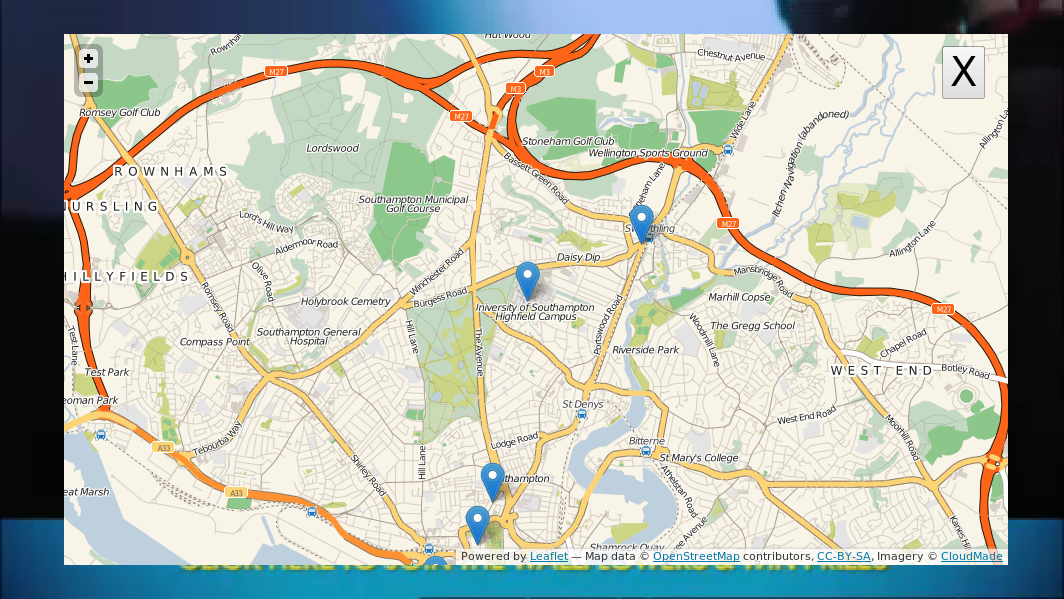
\includegraphics[width=\textwidth,height=0.5\textheight,keepaspectratio]{images/adverts/wallflower-3.png}
		\caption{The Perks of Being a Wallflower film advert, map shown.}
		\label{fig:wallflower3}
	\end{figure}
	
	\begin{figure}[th]
		\centering
		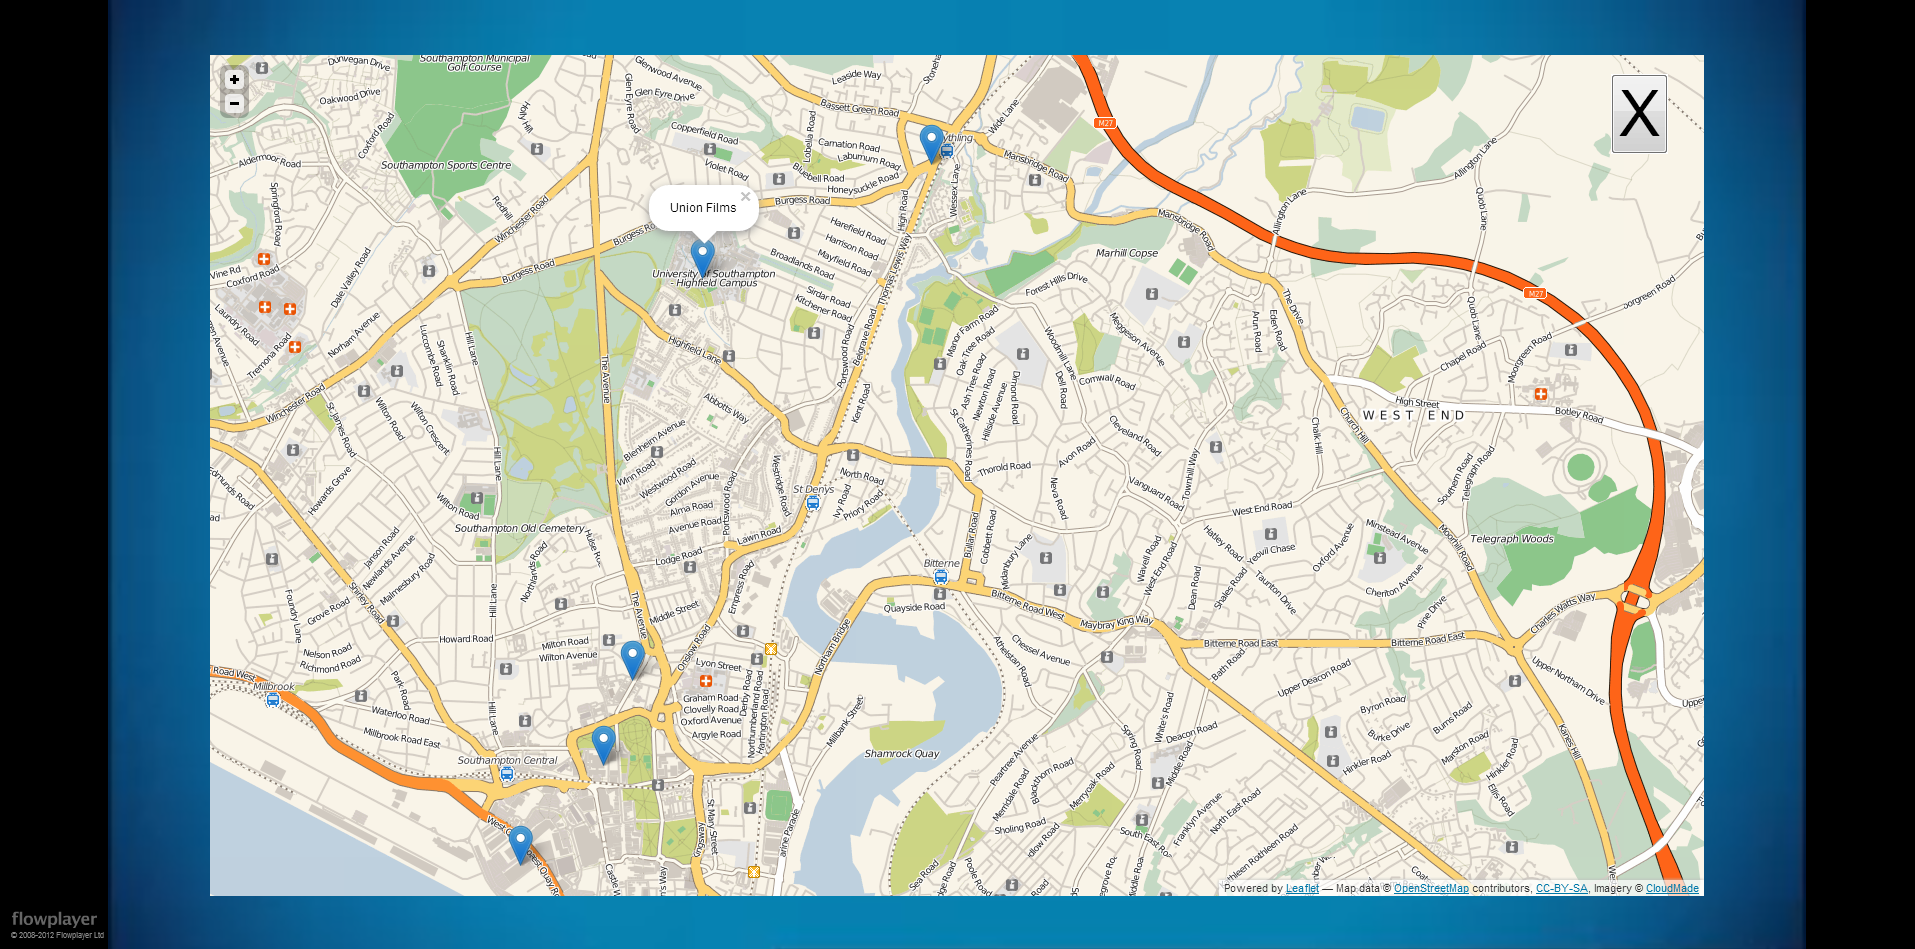
\includegraphics[width=\textwidth,height=0.5\textheight,keepaspectratio]{images/adverts/wallflower-4.png}
		\caption{The Perks of Being a Wallflower film advert, clicked on marker.}
		\label{fig:wallflower4}
	\end{figure}
	
\subsection{Visit Scotland}
	\begin{description}
		\item[On Load]{Grey, semi-transparent bar displayed along the bottom of the screen with the text ``Planning a trip?''. To the right of this is a text box with helper text ``enter your email address'', a button marked ``email me'' and finally a ``X'' button. See \ref{fig:visit_scotland1}.}
		\item[On clicking the ``X'' button]{The grey box fades out.}
		\item[On clicking ``email me'' with an email address in the email text box]{The controls in the bar are removed and replaced with the text ``Thank you''. See \ref{fig:visit_scotland2} and \ref{fig:visit_scotland3}.}
		\item[On Timeout]{Text fades away leaving the advert unobstructed.}
	\end{description}
	
	\begin{figure}[th]
		\centering
		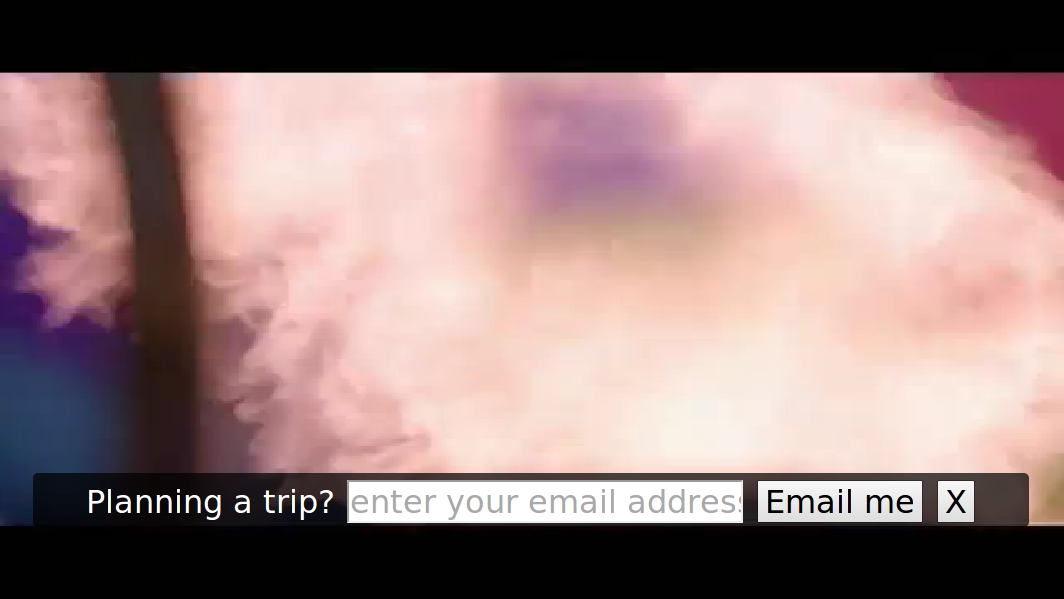
\includegraphics[width=\textwidth,height=0.5\textheight,keepaspectratio]{images/adverts/visit_scotland-1.png}
		\caption{Visit Scotland advert, initial.}
		\label{fig:visit_scotland1}
	\end{figure}
	
	\begin{figure}[th]
		\centering
		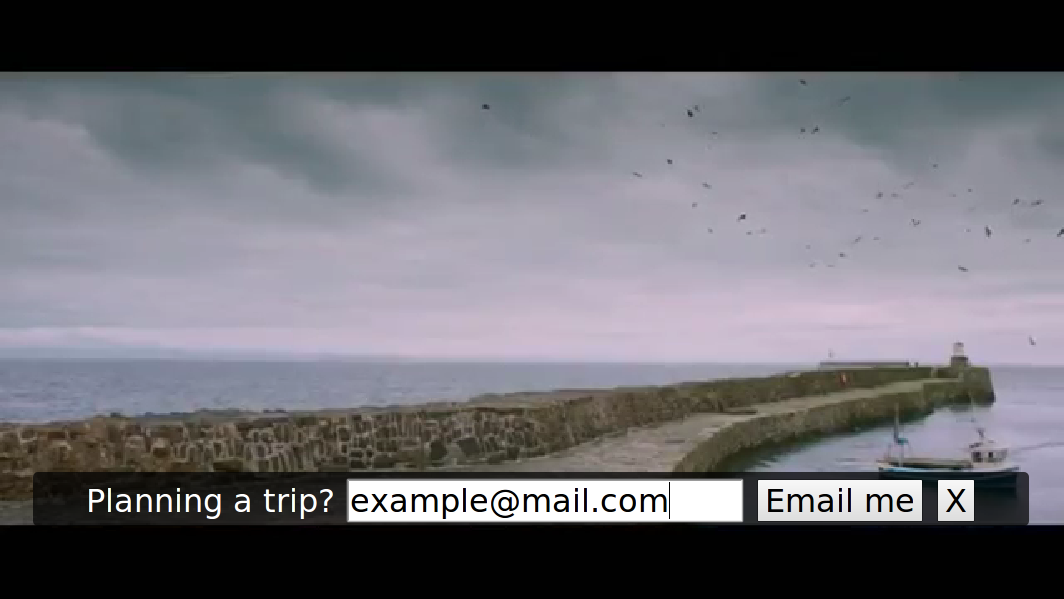
\includegraphics[width=\textwidth,height=0.5\textheight,keepaspectratio]{images/adverts/visit_scotland-2.png}
		\caption{Visit Scotland advert, email entered.}
		\label{fig:visit_scotland2}
	\end{figure}
	
	\begin{figure}[th]
		\centering
		
\includegraphics[width=\textwidth,height=0.5\textheight,keepaspectratio]{images/adverts/visit_scotland-3.png}
		\caption{Visit Scotland advert, email submitted.}
		\label{fig:visit_scotland3}
	\end{figure}